\documentclass{standalone}
\usepackage{tikz}
\usetikzlibrary{patterns, positioning}


\begin{document}
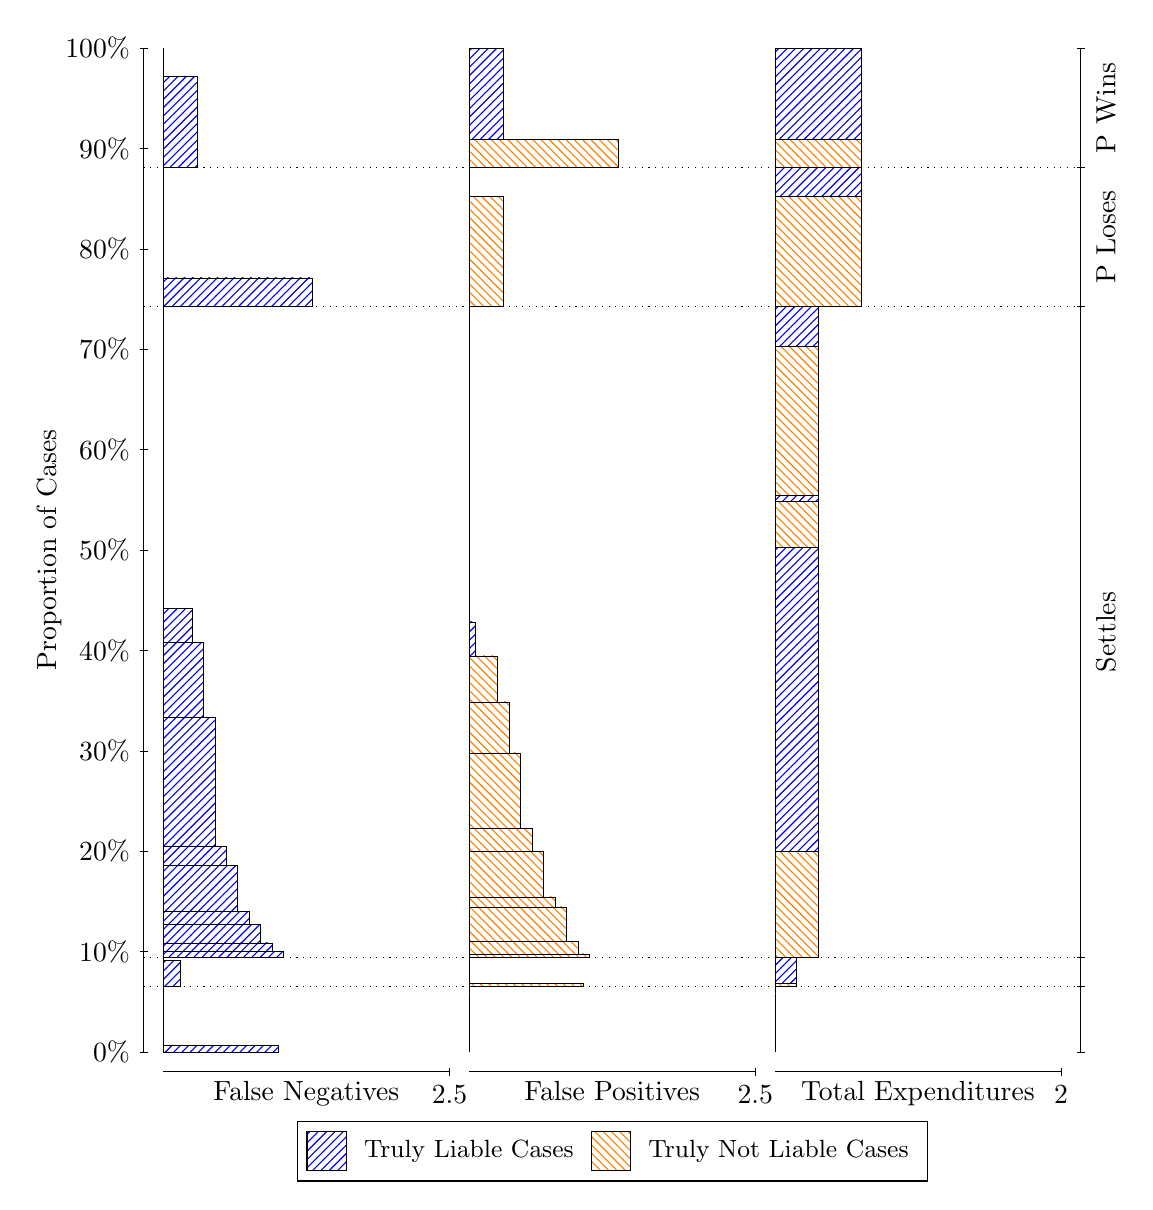
\begin{tikzpicture}
\draw[black, very thin] (1.5,1.75) -- (1.5,14.5);
\node[rotate=90, text=black, anchor=center] at (0.3, 8.125) {Proportion of Cases};
\draw[black, very thin] (1.45,1.75) -- (1.55,1.75);
\node[text=black, anchor=east] at (1.45, 1.75) {0\%};
\draw[black, very thin] (1.45,3.025) -- (1.55,3.025);
\node[text=black, anchor=east] at (1.45, 3.025) {10\%};
\draw[black, very thin] (1.45,4.3) -- (1.55,4.3);
\node[text=black, anchor=east] at (1.45, 4.3) {20\%};
\draw[black, very thin] (1.45,5.575) -- (1.55,5.575);
\node[text=black, anchor=east] at (1.45, 5.575) {30\%};
\draw[black, very thin] (1.45,6.85) -- (1.55,6.85);
\node[text=black, anchor=east] at (1.45, 6.85) {40\%};
\draw[black, very thin] (1.45,8.125) -- (1.55,8.125);
\node[text=black, anchor=east] at (1.45, 8.125) {50\%};
\draw[black, very thin] (1.45,9.4) -- (1.55,9.4);
\node[text=black, anchor=east] at (1.45, 9.4) {60\%};
\draw[black, very thin] (1.45,10.675) -- (1.55,10.675);
\node[text=black, anchor=east] at (1.45, 10.675) {70\%};
\draw[black, very thin] (1.45,11.95) -- (1.55,11.95);
\node[text=black, anchor=east] at (1.45, 11.95) {80\%};
\draw[black, very thin] (1.45,13.225) -- (1.55,13.225);
\node[text=black, anchor=east] at (1.45, 13.225) {90\%};
\draw[black, very thin] (1.45,14.5) -- (1.55,14.5);
\node[text=black, anchor=east] at (1.45, 14.5) {100\%};

\draw[black, very thin] (13.4,1.75) -- (13.4,14.5);
\draw[black, very thin] (13.35,1.75) -- (13.45,1.75);
\node[anchor=west] at (13.35, 1.75) {};
\draw[black, very thin] (13.35,2.5803) -- (13.45,2.5803);
\node[anchor=west] at (13.35, 2.5803) {};
\draw[black, very thin] (13.35,2.9472) -- (13.45,2.9472);
\node[anchor=west] at (13.35, 2.9472) {};
\draw[black, very thin] (13.35,11.219) -- (13.45,11.219);
\node[anchor=west] at (13.35, 11.219) {};
\draw[black, very thin] (13.35,12.981) -- (13.45,12.981);
\node[anchor=west] at (13.35, 12.981) {};
\draw[black, very thin] (13.35,14.5) -- (13.45,14.5);
\node[anchor=west] at (13.35, 14.5) {};

\draw[black, very thin, pattern color=blue, pattern=north east lines] (1.75,1.75) rectangle (3.2033,1.8374);
\draw[black, very thin, pattern color=orange, pattern=north west lines] (1.75,1.8374) rectangle (1.75,2.5803);
\draw[black, very thin, pattern color=blue, pattern=north east lines] (1.75,2.5803) rectangle (1.968,2.909);
\draw[black, very thin, pattern color=orange, pattern=north west lines] (1.75,2.909) rectangle (1.75,2.9472);
\draw[black, very thin, pattern color=blue, pattern=north east lines] (1.75,2.9472) rectangle (3.276,3.0251);
\draw[black, very thin, pattern color=blue, pattern=north east lines] (1.75,3.0251) rectangle (3.1307,3.1366);
\draw[black, very thin, pattern color=blue, pattern=north east lines] (1.75,3.1366) rectangle (2.9853,3.3749);
\draw[black, very thin, pattern color=blue, pattern=north east lines] (1.75,3.3749) rectangle (2.84,3.5381);
\draw[black, very thin, pattern color=blue, pattern=north east lines] (1.75,3.5381) rectangle (2.6947,4.1215);
\draw[black, very thin, pattern color=blue, pattern=north east lines] (1.75,4.1215) rectangle (2.5493,4.3564);
\draw[black, very thin, pattern color=blue, pattern=north east lines] (1.75,4.3564) rectangle (2.404,6.0041);
\draw[black, very thin, pattern color=blue, pattern=north east lines] (1.75,6.0041) rectangle (2.2587,6.9552);
\draw[black, very thin, pattern color=blue, pattern=north east lines] (1.75,6.9552) rectangle (2.1133,7.3865);
\draw[black, very thin, pattern color=orange, pattern=north west lines] (1.75,7.3865) rectangle (1.75,11.219);
\draw[black, very thin, pattern color=blue, pattern=north east lines] (1.75,11.219) rectangle (3.6393,11.582);
\draw[black, very thin, pattern color=orange, pattern=north west lines] (1.75,11.582) rectangle (1.75,12.981);
\draw[black, very thin, pattern color=blue, pattern=north east lines] (1.75,12.981) rectangle (2.186,14.139);
\draw[black, very thin, pattern color=orange, pattern=north west lines] (1.75,14.139) rectangle (1.75,14.5);
\draw[black, very thin, pattern color=orange, pattern=north west lines] (5.6333,1.75) rectangle (5.6333,2.493);
\draw[black, very thin, pattern color=blue, pattern=north east lines] (5.6333,2.493) rectangle (5.6333,2.5803);
\draw[black, very thin, pattern color=orange, pattern=north west lines] (5.6333,2.5803) rectangle (7.0867,2.6186);
\draw[black, very thin, pattern color=blue, pattern=north east lines] (5.6333,2.6186) rectangle (5.6333,2.9472);
\draw[black, very thin, pattern color=orange, pattern=north west lines] (5.6333,2.9472) rectangle (7.1593,2.9951);
\draw[black, very thin, pattern color=orange, pattern=north west lines] (5.6333,2.9951) rectangle (7.014,3.1528);
\draw[black, very thin, pattern color=orange, pattern=north west lines] (5.6333,3.1528) rectangle (6.8687,3.5925);
\draw[black, very thin, pattern color=orange, pattern=north west lines] (5.6333,3.5925) rectangle (6.7233,3.7207);
\draw[black, very thin, pattern color=orange, pattern=north west lines] (5.6333,3.7207) rectangle (6.578,4.3005);
\draw[black, very thin, pattern color=orange, pattern=north west lines] (5.6333,4.3005) rectangle (6.4327,4.3022);
\draw[black, very thin, pattern color=orange, pattern=north west lines] (5.6333,4.3022) rectangle (6.4327,4.5895);
\draw[black, very thin, pattern color=orange, pattern=north west lines] (5.6333,4.5895) rectangle (6.2873,5.549);
\draw[black, very thin, pattern color=orange, pattern=north west lines] (5.6333,5.549) rectangle (6.142,6.1965);
\draw[black, very thin, pattern color=orange, pattern=north west lines] (5.6333,6.1965) rectangle (5.9967,6.7798);
\draw[black, very thin, pattern color=blue, pattern=north east lines] (5.6333,6.7798) rectangle (5.706,7.2112);
\draw[black, very thin, pattern color=blue, pattern=north east lines] (5.6333,7.2112) rectangle (5.6333,11.219);
\draw[black, very thin, pattern color=orange, pattern=north west lines] (5.6333,11.219) rectangle (6.0693,12.619);
\draw[black, very thin, pattern color=blue, pattern=north east lines] (5.6333,12.619) rectangle (5.6333,12.981);
\draw[black, very thin, pattern color=orange, pattern=north west lines] (5.6333,12.981) rectangle (7.5227,13.343);
\draw[black, very thin, pattern color=blue, pattern=north east lines] (5.6333,13.343) rectangle (6.0693,14.5);
\draw[black, very thin, pattern color=orange, pattern=north west lines] (9.5167,1.75) rectangle (9.5167,2.493);
\draw[black, very thin, pattern color=blue, pattern=north east lines] (9.5167,2.493) rectangle (9.5167,2.5803);
\draw[black, very thin, pattern color=orange, pattern=north west lines] (9.5167,2.5803) rectangle (9.7892,2.6186);
\draw[black, very thin, pattern color=blue, pattern=north east lines] (9.5167,2.6186) rectangle (9.7892,2.9472);
\draw[black, very thin, pattern color=orange, pattern=north west lines] (9.5167,2.9472) rectangle (10.062,4.3022);
\draw[black, very thin, pattern color=blue, pattern=north east lines] (9.5167,4.3022) rectangle (10.062,8.1574);
\draw[black, very thin, pattern color=orange, pattern=north west lines] (9.5167,8.1574) rectangle (10.062,8.7407);
\draw[black, very thin, pattern color=blue, pattern=north east lines] (9.5167,8.7407) rectangle (10.062,8.8186);
\draw[black, very thin, pattern color=orange, pattern=north west lines] (9.5167,8.8186) rectangle (10.062,10.713);
\draw[black, very thin, pattern color=blue, pattern=north east lines] (9.5167,10.713) rectangle (10.062,11.219);
\draw[black, very thin, pattern color=orange, pattern=north west lines] (9.5167,11.219) rectangle (10.607,12.619);
\draw[black, very thin, pattern color=blue, pattern=north east lines] (9.5167,12.619) rectangle (10.607,12.981);
\draw[black, very thin, pattern color=orange, pattern=north west lines] (9.5167,12.981) rectangle (10.607,13.343);
\draw[black, very thin, pattern color=blue, pattern=north east lines] (9.5167,13.343) rectangle (10.607,14.5);
\draw[black, dotted] (1.5,2.5803) -- (13.4,2.5803);
\draw[black, dotted] (1.5,2.9472) -- (13.4,2.9472);
\draw[black, dotted] (1.5,11.219) -- (13.4,11.219);
\draw[black, dotted] (1.5,12.981) -- (13.4,12.981);
\draw[black, very thin] (1.75,1.5) -- (5.3833,1.5);
\node[text=black, anchor=north] at (3.5667, 1.5) {False Negatives};
\draw[black, very thin] (5.3833,1.45) -- (5.3833,1.55);
\node[text=black, anchor=north] at (5.3833, 1.45) {2.5};

\draw[black, very thin] (5.6333,1.5) -- (9.2667,1.5);
\node[text=black, anchor=north] at (7.45, 1.5) {False Positives};
\draw[black, very thin] (9.2667,1.45) -- (9.2667,1.55);
\node[text=black, anchor=north] at (9.2667, 1.45) {2.5};

\draw[black, very thin] (9.5167,1.5) -- (13.15,1.5);
\node[text=black, anchor=north] at (11.333, 1.5) {Total Expenditures};
\draw[black, very thin] (13.15,1.45) -- (13.15,1.55);
\node[text=black, anchor=north] at (13.15, 1.45) {2};



\node[text=black, centered, rotate=90] at (13.72, 7.0832) {Settles};
\node[text=black, centered, rotate=90] at (13.72, 12.1) {P Loses};
\node[text=black, centered, rotate=90] at (13.72, 13.741) {P Wins};

\draw (7.449999999999999,1.5) node[draw=none] (baseCoordinate) {};
\begin{scope}[align=center]
        \matrix[scale=0.5, draw=black, below=0.5cm of baseCoordinate, nodes={draw}, column sep=0.1cm]{
            \node[rectangle, draw, minimum width=0.5cm, minimum height=0.5cm, pattern color=blue, pattern=north east lines] {}; &
            \node[draw=none, font=\small, text=black] (B) {Truly Liable Cases}; &
            \node[rectangle, draw, minimum width=0.5cm, minimum height=0.5cm, pattern color=orange, pattern=north west lines] {}; &
            \node[draw=none, font=\small, text=black] (B) {Truly Not Liable Cases}; \\
            };
\end{scope}

\end{tikzpicture}
\end{document}